\chapter{Fonctions}
\section*{}
Excel dispose un ensemble d'outils pour réaliser des calculs de maniere dynamique ou static. La performance de cette logiciel permet de calculer le resultat des milliers de cellules grace à une fonction définie(écrite par l'utilisateur) ou prédéfinie( existe déja).

\begin{center}  
	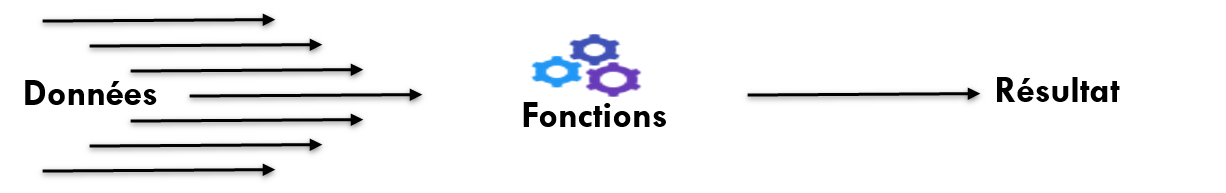
\includegraphics[scale=0.2,width= \linewidth]{img/fonctions}
	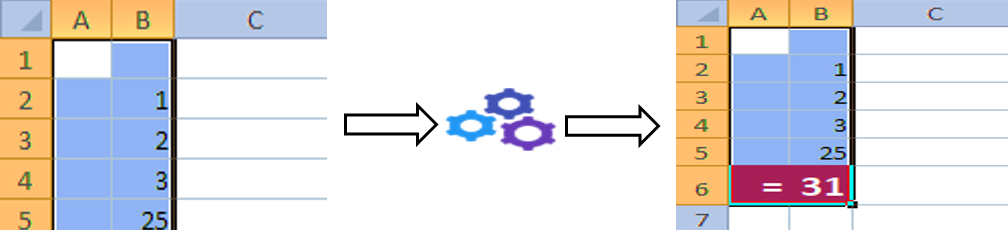
\includegraphics[scale=0.2,width= \linewidth]{img/fonctions2}
\end{center}

\section{Fonctions Arithmétique}
\textbf{{{ Méthode 1}}}
\begin{center}  
	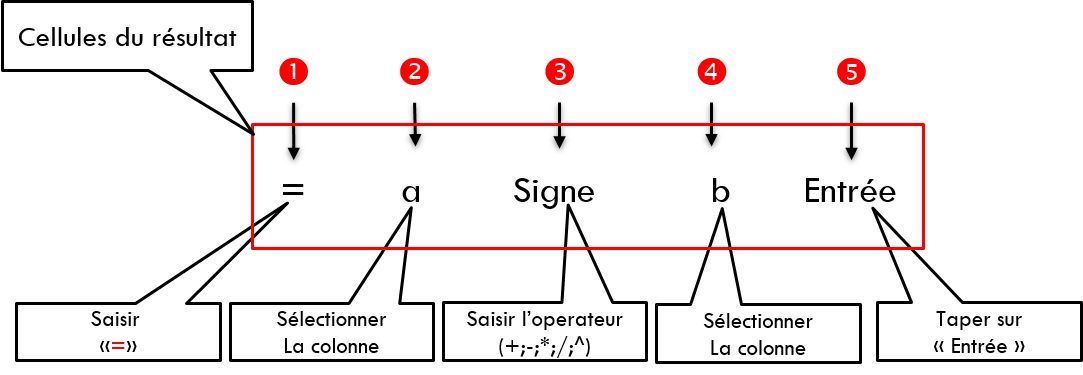
\includegraphics[scale=0.2,width= \linewidth]{img/arithmetique1} 
	\captionof{figure}{Syntaxe d'une formule Arithmétique} 
\end{center}
\begin{Exemple}
\end{Exemple}
\begin{center}  
	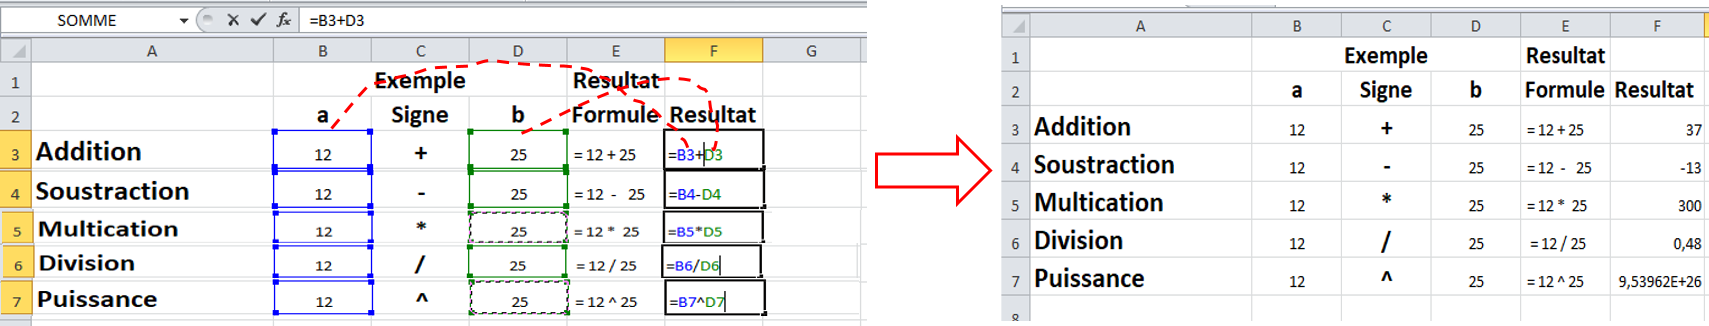
\includegraphics[scale=0.2,width= \linewidth]{img/arithmetique2} 
	\captionof{figure}{Operateur Arithmétique } 
\end{center}
\newpage
\textbf{{{ Méthode 2}}}

\begin{center}  
	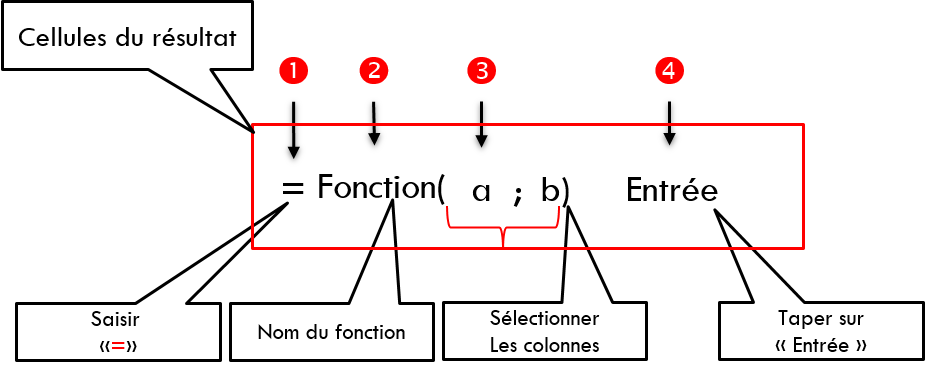
\includegraphics[scale=0.2,width= \linewidth]{img/arithmetique3} 
\end{center}

\begin{Exemple}
\end{Exemple}
\begin{center}  
	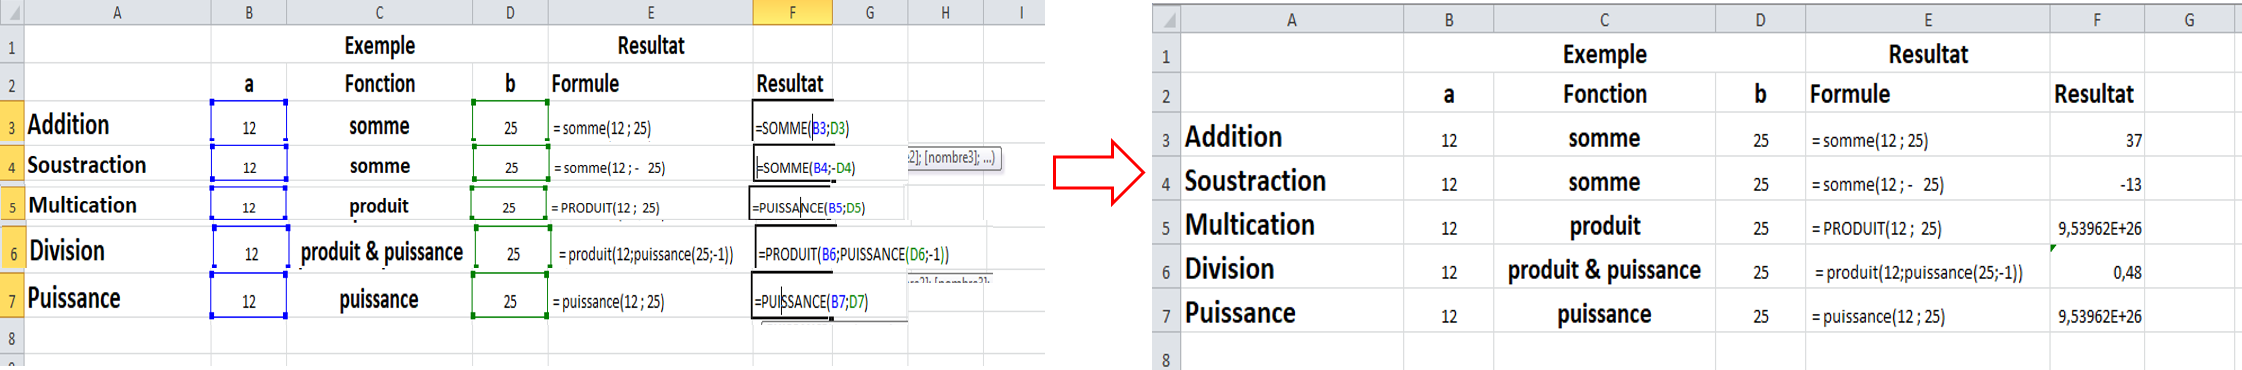
\includegraphics[scale=0.2,width= \linewidth]{img/fonctions3} 
	\captionof{figure}{Operateur Arithmétique fonction prédefinie} 
\end{center}

\section{Série d'Exercices}

\begin{exercice}\label{ex8}
	Consignes 
	\begin{enumerate}		
		\item  Saisissez le tableau  de la Figure (\ref{exo8}) à l'aide du saisie rapide.  				
		\item  Mettez la mise en forme  du tableau.
		\item  Calculez la somme total des valeurs.
	\end{enumerate}	
\end{exercice}
\begin{figure}[H]
	\centering
	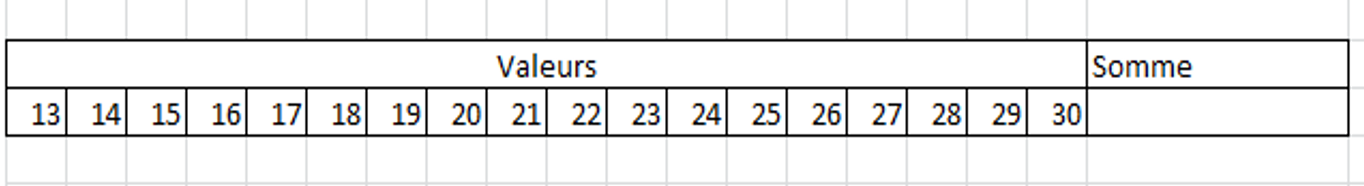
\includegraphics[scale=0.2,width= \linewidth]{img/ex08}
	\captionof{figure}{Exercice \ref{ex8}} \label{exo8}
\end{figure}

\begin{exercice}\label{ex9}
	Consignes 
	\begin{enumerate}		
		\item  Saisissez le tableau  de la Figure (\ref{exo9}) à l'aide du saisie rapide.  				
		\item  Mettez la mise en forme  du tableau.
		\item  Calculez le produit total des valeurs.
	\end{enumerate}	
\end{exercice}
\begin{figure}[H]
	\centering
	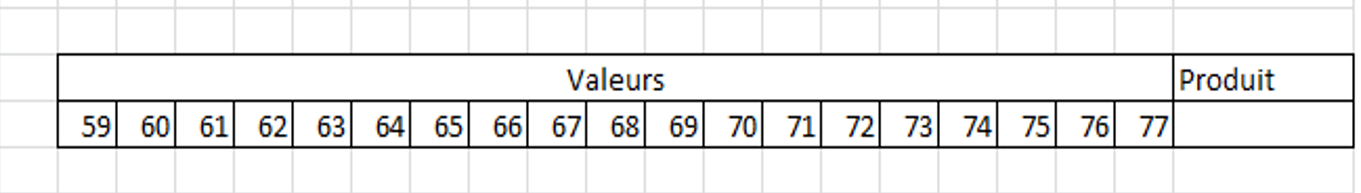
\includegraphics[scale=0.2,width= \linewidth]{img/ex09}
	\captionof{figure}{Exercice \ref{ex9}} \label{exo9}
\end{figure}

\begin{exercice}\label{ex10}
	Consignes 
	\begin{enumerate}		
		\item  Saisissez le tableau  de la Figure (\ref{exo10}).  				
		\item  Mettez la mise en forme  du tableau.
		\item  Calculez la Somme Note,  tel que Somme Note=Note1 + Note2+Note3.
		\item  Calculez la Moyenne Matière,  tel que Moyen Matière= (Somme Note) / (Nombre de Notes).
		\item  Calculez la Note Matière ,  Note Matière = (Moyen Matière)* Coefficient.
		\item  Calculez la Moyenne,  tel que Moyenne= (Total note Matière)/ (Total Coefficient).
		\subitem NB: Total X= somme des éléments de X
		\item Centrer les valeurs calculées			
	\end{enumerate}	
\end{exercice}
\begin{figure}[H]
	\centering
	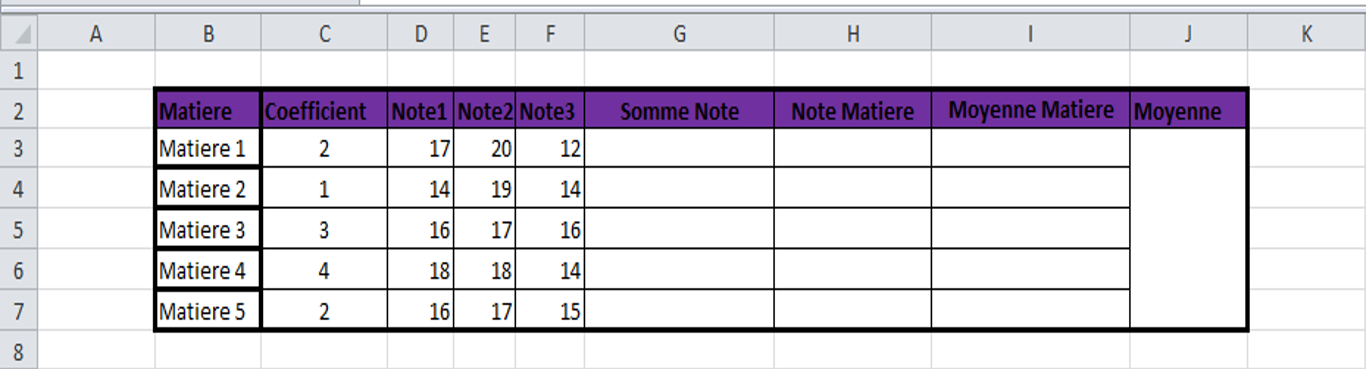
\includegraphics[scale=0.2,width= \linewidth]{img/ex010}
	\captionof{figure}{Exercice \ref{ex10}} \label{exo10}
\end{figure}

\section{Autres Fonctions}
\subsection{Fonction de Recherche: minimum \& maximum }
La fonction de recherche (minimum \& maximum) consiste à trouver la valeur minimum(maximum) sur un ensemble de valeurs données, pour se faire
\begin{center}  
	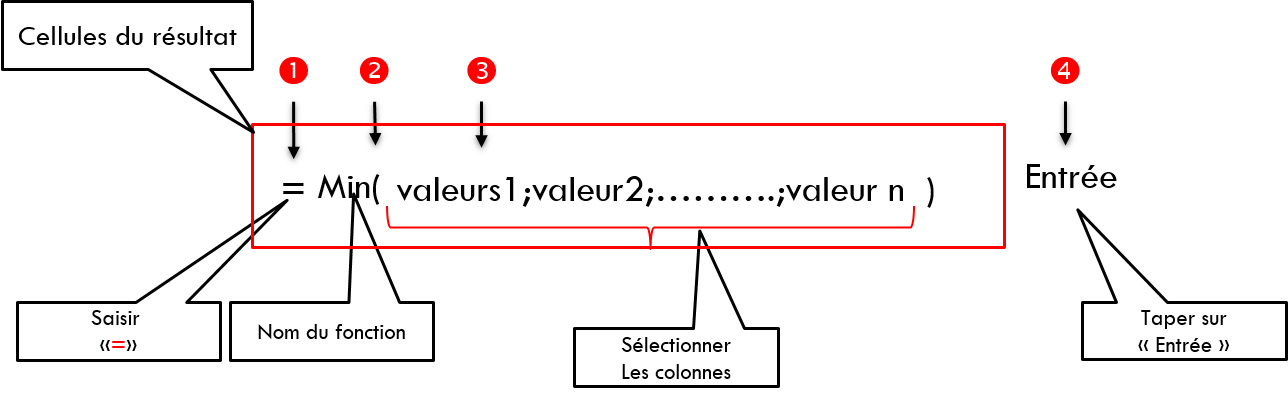
\includegraphics[scale=0.2,width= \linewidth]{img/minimum} 
	\captionof{figure}{Fonction minimum} 
\end{center}

\begin{center}  
	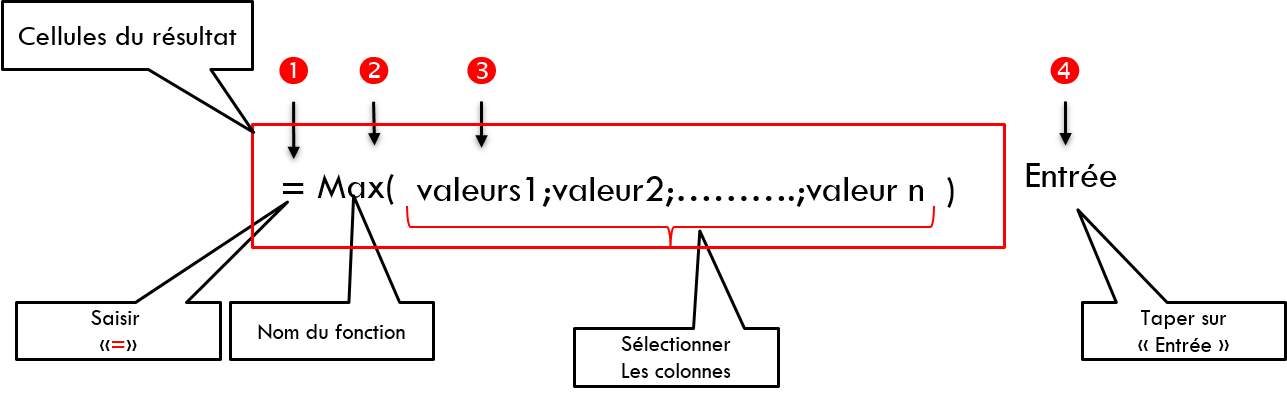
\includegraphics[scale=0.2,width= \linewidth]{img/maximum} 
	\captionof{figure}{Fonction maximum} 
\end{center}

\section{Série d'Exercices}

\begin{exercice}\label{ex11}
	Consignes 
	\begin{enumerate}		
		\item  Saisissez le tableau  de la Figure (\ref{exo11}) à l'aide du saisie rapide.  				
		\item  Mettez la mise en forme  du tableau.
		\item  Calculez le minimum des valeurs du tableau.
	\end{enumerate}	
\end{exercice}
\begin{figure}[H]
	\centering
	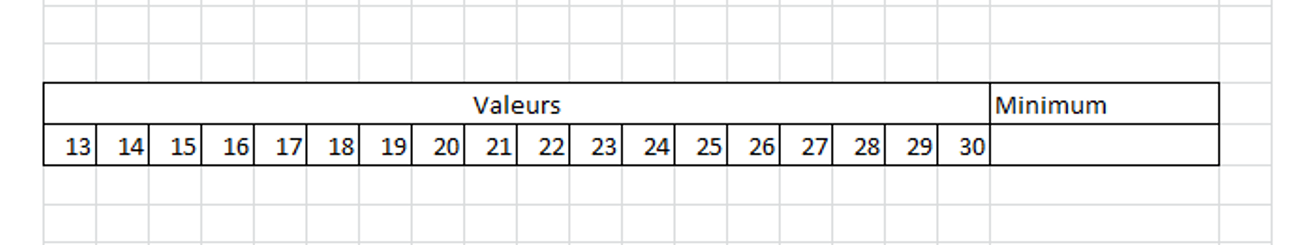
\includegraphics[scale=0.2,width= \linewidth]{img/ex011}
	\captionof{figure}{Exercice \ref{ex11}} \label{exo11}
\end{figure}

\begin{exercice}\label{ex12}
	Consignes 
	\begin{enumerate}		
		\item  Saisissez le tableau  de la Figure (\ref{exo12}) à l'aide du saisie rapide.  				
		\item  Mettez la mise en forme  du tableau.
		\item  Calculez le maximum des valeurs du tableau.
	\end{enumerate}	
\end{exercice}
\begin{figure}[H]
	\centering
	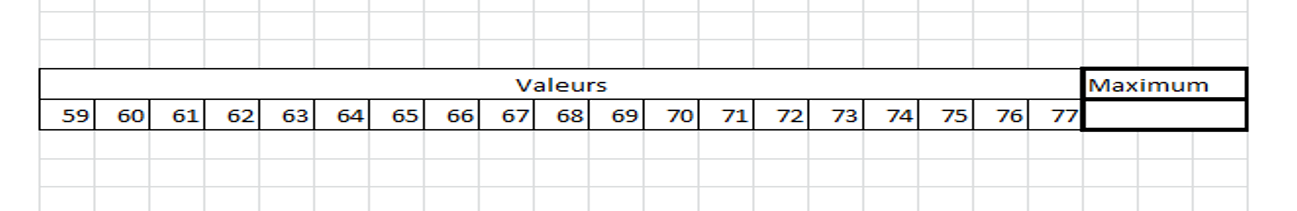
\includegraphics[scale=0.2,width= \linewidth]{img/ex012}
	\captionof{figure}{Exercice \ref{ex12}} \label{exo12}
\end{figure}

\begin{exercice}\label{ex13}
	Consignes 
	\begin{enumerate}		
		\item  Saisissez le tableau  de la Figure (\ref{exo13}).  				
		\item  Mettez la mise en forme  du tableau.
		\item  Calculez la Somme Note,  tel que Somme Note=Note1 + Note2+Note3.
		\item  Calculez la Moyenne Matière,  tel que Moyen Matière= (Somme Note) / (Nombre de Notes).
		\item  Calculez la Note Matière ,  Note Matière = (Moyen Matière)* Coefficient.
		\item  Calculez la Moyenne,  tel que Moyenne= (Total note Matière)/ (Total Coefficient).
		\subitem NB: Total X= somme des éléments de X
		\item Calculer le \textbf{maximum1} et \textbf{minimum1} des notes
		\item Calculer le \textbf{maximum2} et \textbf{minimum2} de chaque colonne
		\item Centrer les valeurs calculées			
	\end{enumerate}	
\end{exercice}
\begin{figure}[H]
	\centering
	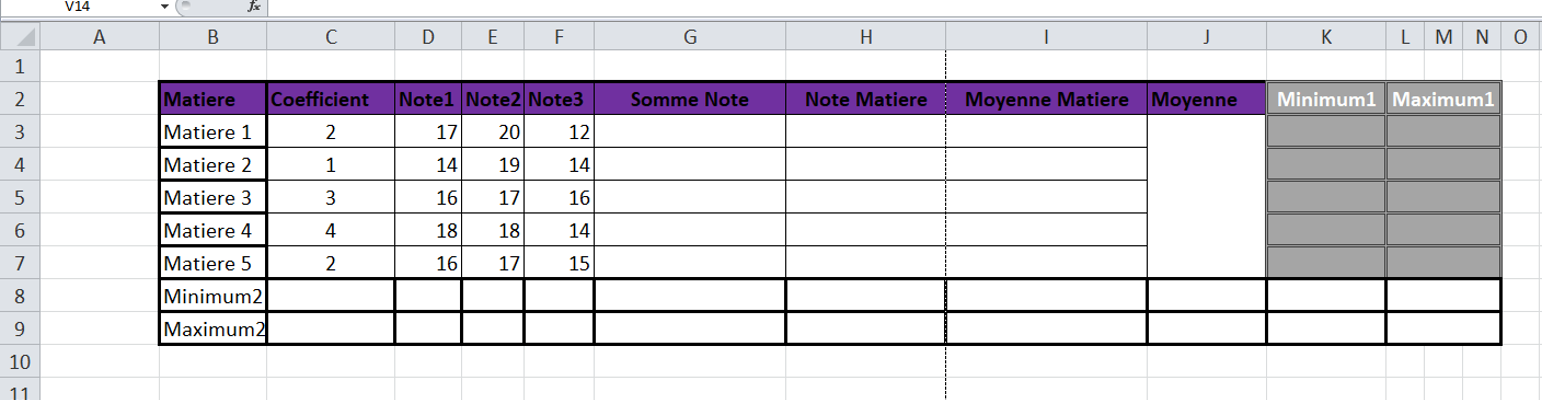
\includegraphics[scale=0.2,width= \linewidth]{img/ex013}
	\captionof{figure}{Exercice \ref{ex13}} \label{exo13}
\end{figure}


\section{Les conditions}
Les conditions permet de donner des ordres sous certains contrainte. Par exemple si telle cellule vaut \textbf{X}, alors fais \textbf{ceci},	sinon, fais	
  \textbf{cela}	

\subsection{Les Conditions Simples}
\begin{figure}[H]
	\centering
	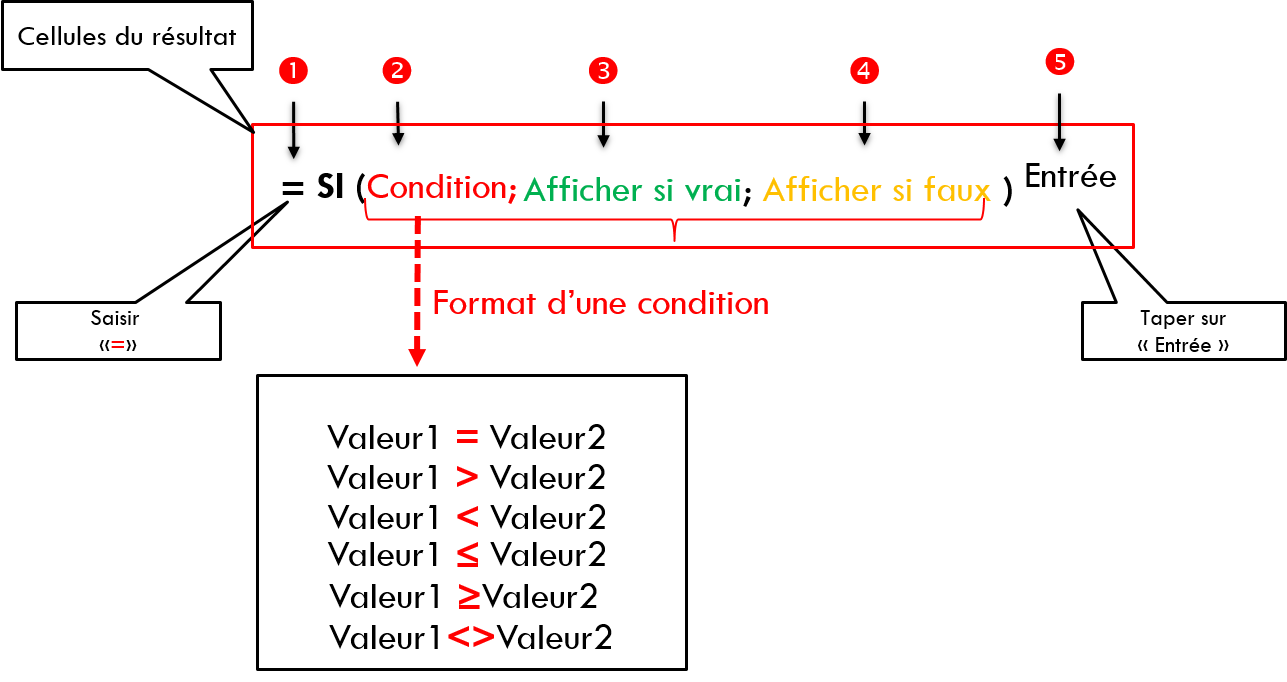
\includegraphics[scale=0.2,width= \linewidth]{img/conditions_syntaxt}
	\captionof{figure}{Syntaxe d'une condition simple}
\end{figure}

\begin{Exemple}
	Cette exemple illustre l'utilisation des conditions simples
\end{Exemple}
\begin{center}  
	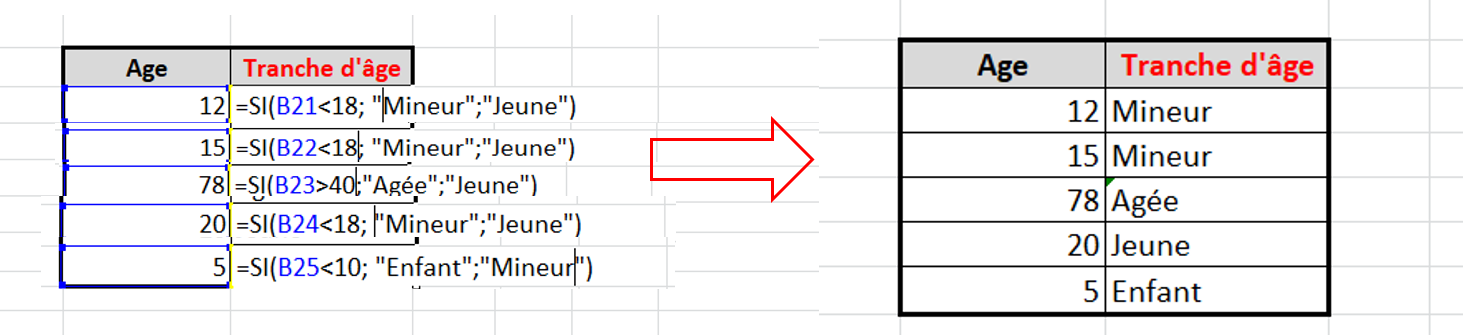
\includegraphics[scale=0.2,width=\linewidth]{img/condition_exemple}
	\captionof{figure}{Exemple condition simple} 
\end{center}

\subsection{Les Conditions Multiples}
Les conditions simples permet de tester que deux (02) valeurs, Il est alors impossible de tester une tranche de valeurs. L'utilisation des operateurs logique permet de remedier à ce problèmes.

\begin{figure}[H]
	\centering
	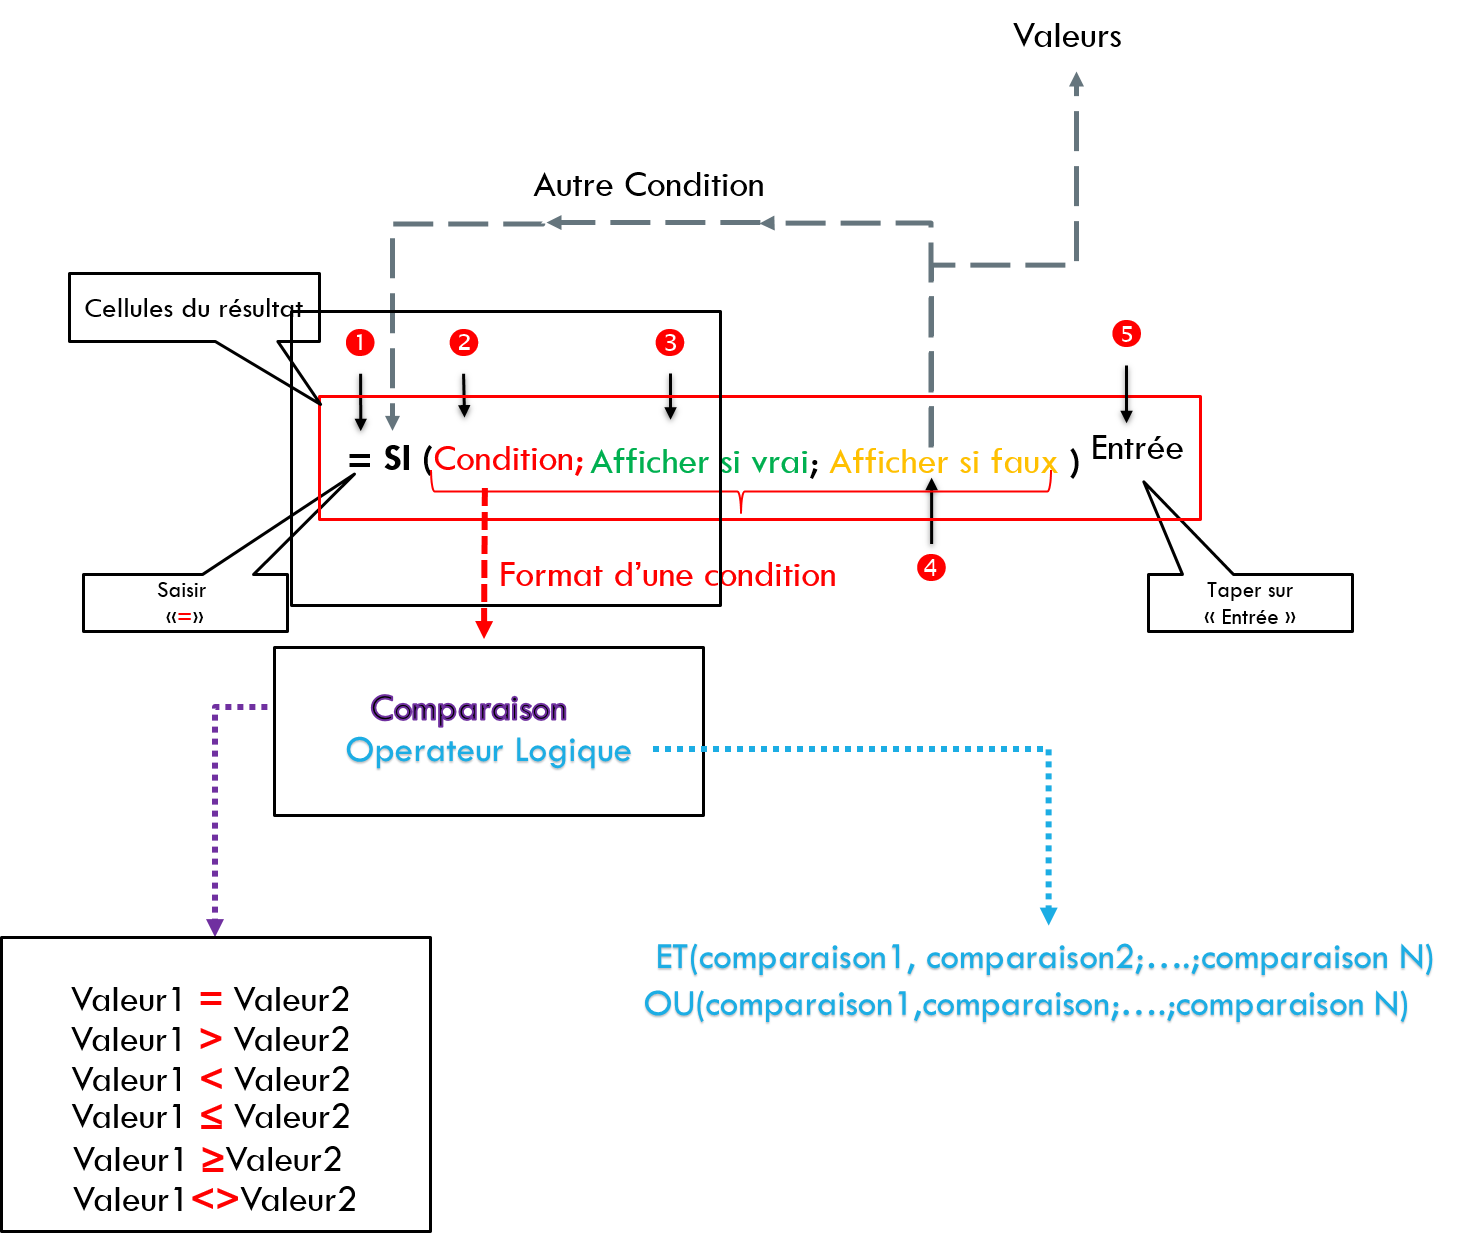
\includegraphics[scale=0.2,width= \linewidth]{img/condition_multiple}
	\captionof{figure}{Syntaxe condition multiple}
\end{figure}

\begin{Exemple}
	Cette exemple illustre l'utilisation des conditions multiples
\end{Exemple}
\begin{center}  
	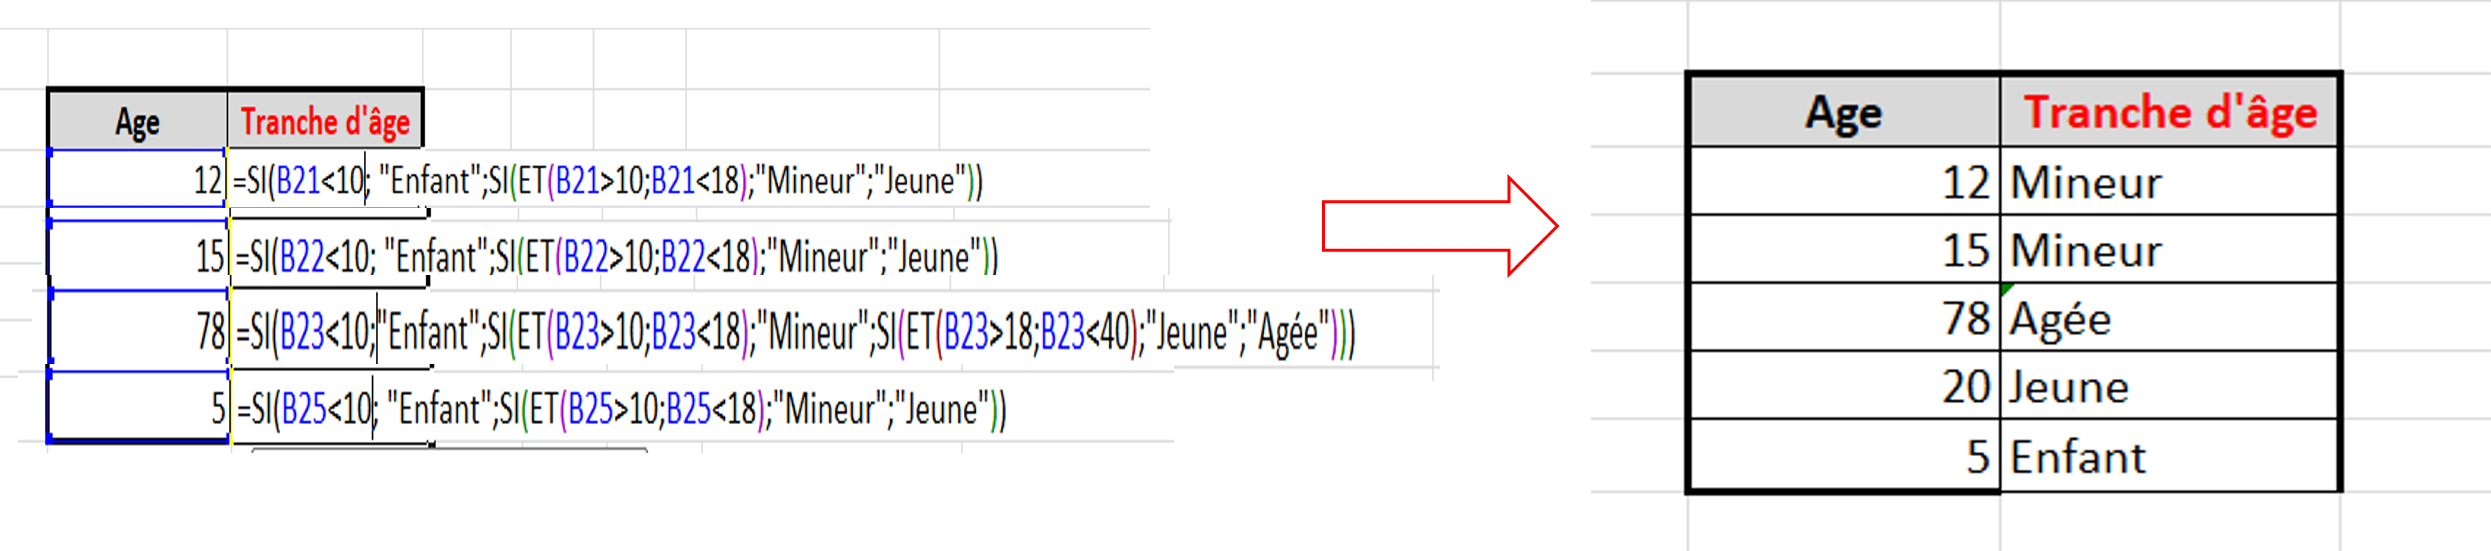
\includegraphics[scale=0.2,width=\linewidth]{img/condition_multiple_exemple}
	\captionof{figure}{Exemple condition multiple} 
\end{center}

\section{Série d'Exercices}

\begin{exercice} 
	Consignes 
	\begin{enumerate}		
		\item  Saisissez le tableau  de la Figure (\ref{exo14}).  				
		\item  Mettez la mise en forme  du tableau.
		\item  Le Restants à livrer, tel que Restants à livrer= mod(colonne\_Commande;colonne\_livraison).
		\item  Calculer le total de chaque colonne.
	\end{enumerate}	
\end{exercice}
\begin{center}  
	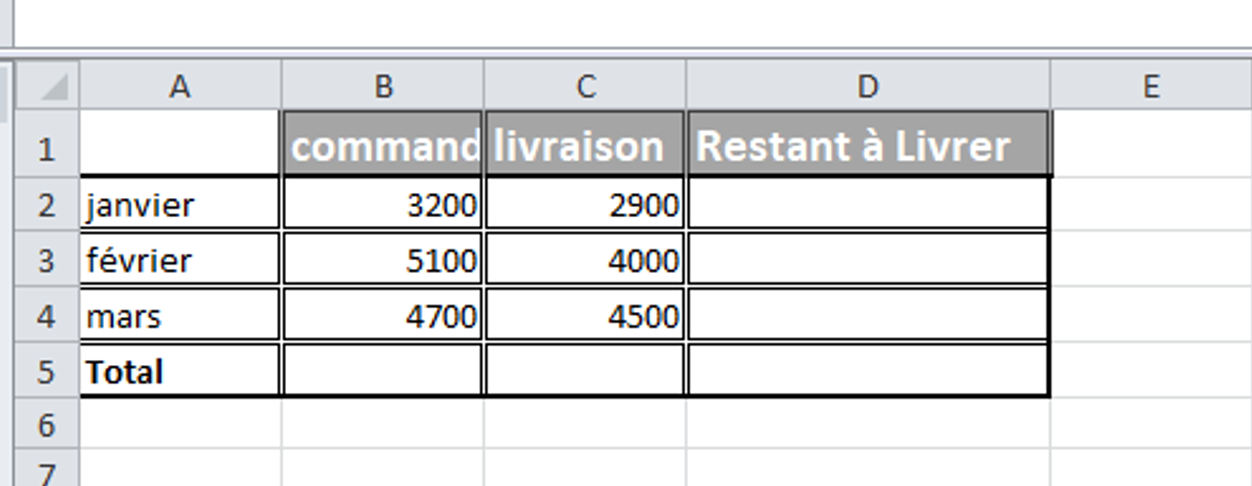
\includegraphics[scale=0.2,width= \linewidth]{img/ex014} 
	\captionof{figure}{ }\label{exo14}
\end{center}

\begin{exercice} 
	Consignes 
	\begin{enumerate}		
		\item  Saisissez le tableau  de la Figure (\ref{exo15}).  				
		\item  Mettez la mise en forme  du tableau.
		\item Calculez la commission a payé sachant que si la vente depasse 500 alors \textbf{7 Euros} doit etre payée, une fois doublée elle sera donc payée \textbf{14 Euros} sinon \textbf{aucune commission}.
	\end{enumerate}	
\end{exercice}
\begin{center}  
	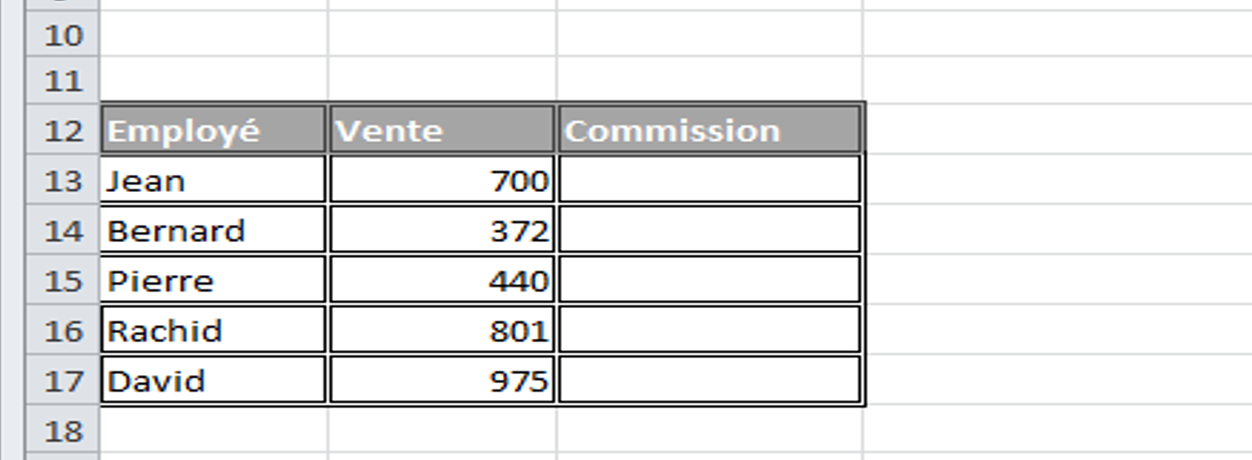
\includegraphics[scale=0.2,width= \linewidth]{img/ex015} 
	\captionof{figure}{ }\label{exo15}
\end{center}

\begin{exercice} 
	Consignes 
	\begin{enumerate}		
		\item  Saisissez le tableau  de la Figure (\ref{exo15}).  				
		\item  Mettez la mise en forme  du tableau.
		\item Calculez CA TTC.
		\item Calculez Com.
	\end{enumerate}	
\begin{description}
	\item[CA TTC  =]   CA HT  * (1 +  Taux  taxe). 
	\item[Com   =]     CA HT  * (1 +  Taux Com . 
\end{description}
\end{exercice}
\begin{center}  
	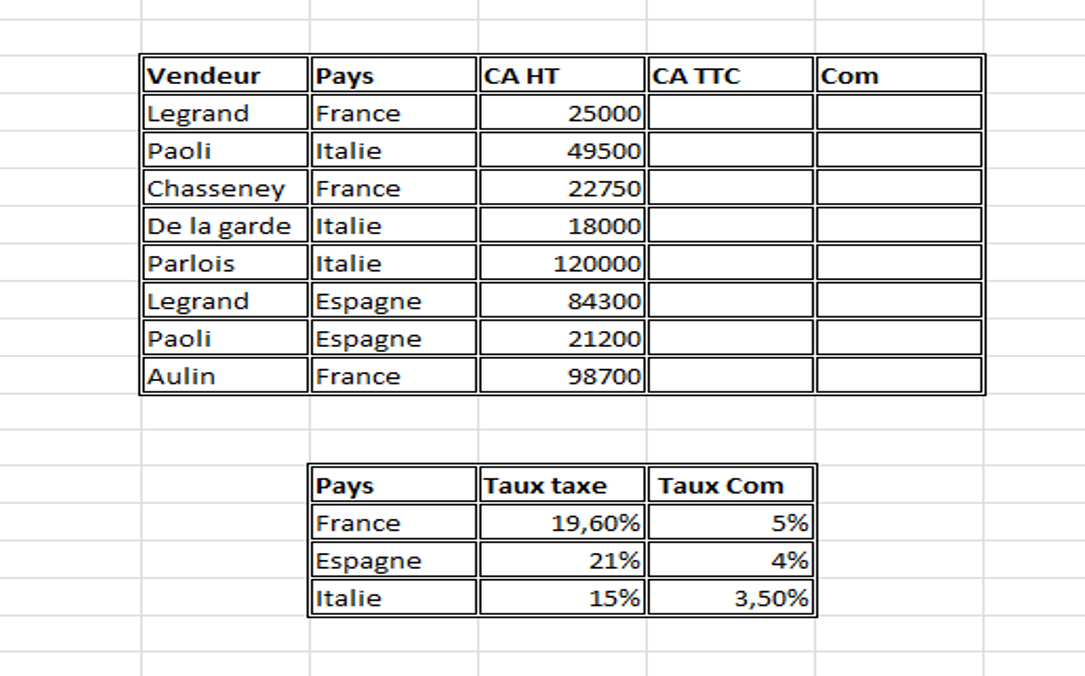
\includegraphics[scale=0.2,width= \linewidth]{img/ex016} 
	\captionof{figure}{ }\label{exo15}
\end{center}
\section{Mise en forme conditionnelle}
